% 2026_national_paper_1_q15_fig1: 直三棱柱 ABC-A1B1C1，D 为 AB 中点，E 为 AC1 中点
\usetikzlibrary{calc}
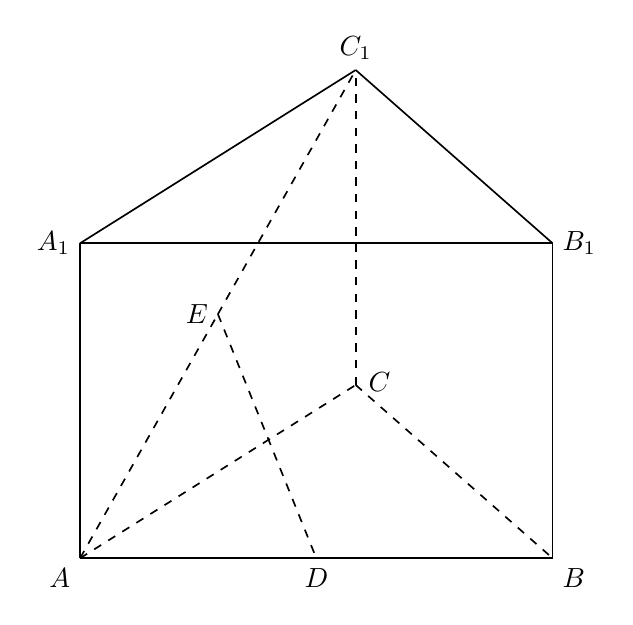
\begin{tikzpicture}[x=1cm,y=1cm,line width=.6pt]
  \coordinate (A) at (0,0);
  \coordinate (B) at (6,0);
  \coordinate (D) at (3,0);
  \coordinate (C) at (3.5,2.2);
  \coordinate (A1) at (0,4);
  \coordinate (B1) at (6,4);
  \coordinate (C1) at (3.5000000000,6.2000000000);
  \coordinate (E) at (1.7500000000,3.1000000000);
  % 底面：AB 可见，AC/BC 遮挡
  \draw (A) -- (B);
  \draw[dashed] (A) -- (C);
  \draw[dashed] (C) -- (B);
  % 侧棱：AA1/BB1 可见，CC1 遮挡
  \draw (A) -- (A1);
  \draw (B) -- (B1);
  \draw[dashed] (C) -- (C1);
  % 顶面
  \draw (A1) -- (B1);
  \draw (A1) -- (C1);
  \draw (B1) -- (C1);
  % 连线：A-C1（含 E），E-D
  \draw[dashed] (A) -- (E);
  \draw[dashed] (E) -- (C1);
  \draw[dashed] (E) -- (D);
  % 标签
  \node[below left,font=\normalsize] at (A) {$A$};
  \node[below right,font=\normalsize] at (B) {$B$};
  \node[below,font=\normalsize] at (D) {$D$};
  \node[right,font=\normalsize,xshift=1.0pt,yshift=1.0pt] at (C) {$C$};
  \node[left,font=\normalsize] at (A1) {$A_1$};
  \node[right,font=\normalsize] at (B1) {$B_1$};
  \node[above,font=\normalsize] at (C1) {$C_1$};
  \node[left,font=\normalsize] at (E) {$E$};
\end{tikzpicture}
